\documentclass[11pt]{article} % 10 = trop de trucs à dire; 11 = joli; 12 = il y a du vide à combler
\setcounter{secnumdepth}{2}

%% Packages -------------------------------------------------------------------
\RequirePackage[english]{babel} % Document's language
\RequirePackage[utf8]{inputenc} % Special characters
\RequirePackage[section]{placeins}%Pour placement de section
\RequirePackage[T1]{fontenc} %Quelques lettres qui sont pas inclus dans UTF-8
\RequirePackage{mathtools} %Paquet pour des équations et symboles mathématiques
\RequirePackage{siunitx} %Pour écrire avec la notation scientifique (Ex.: \num{2e+9})
\usepackage{amsmath}
\usepackage{amssymb}
\RequirePackage{float} %Pour placement d'images
\RequirePackage{graphicx} %Paquet pour insérer des images
\RequirePackage[justification=centering]{caption} %Pour les légendes centralisées
\RequirePackage{subcaption}
\RequirePackage{wallpaper}
\RequirePackage{nomencl}
%\makenomenclature
\RequirePackage{fancyhdr}
%\pagestyle{fancy}
%\fancyheadoffset{1cm}
%\setlength{\headheight}{2cm}
\RequirePackage{url}
\RequirePackage[hidelinks]{hyperref}%Paquet pour insérer légendes dans des sous-figures comme Figure 1a, 1b
\RequirePackage[left=2.5cm,right=2.5cm,top=2cm,bottom=3.5cm]{geometry} 
%Configuration de la page: pour un truc ou il faut de la place, on prend [left=2.5cm,right=2.5cm,top=2cm,bottom=3.5cm], mais quand il faut du vide, [margin=1.5in] 
\usepackage{ragged2e}
\usepackage{blindtext}
\usepackage{qtree}
\usepackage{array}
\usepackage{enumitem}


\DeclareMathOperator\supp{supp}
\DeclareMathOperator\Z{\mathbb{Z}}
\DeclareMathOperator\R{\mathbb{R}}
\DeclareMathOperator\Oo{\mathcal{O}}
\DeclareMathOperator\Nn{\mathcal{N}}



\begin{document}

\begin{titlepage}
\centering

\includegraphics[width=0.5\textwidth]{imgs/mva.png}
\par\vspace{1cm}

{\scshape\LARGE Rémi Ouazan \\ Deformables \& Geodesics \par} 
\vspace{0.5cm}

\rule{\linewidth}{0.2 mm} \\[0.4 cm]
{\huge\bfseries Analyse : Deep Eikonal Solver \par} \
\rule{\linewidth}{0.2 mm} \\[1.0 cm]

\tableofcontents

\end{titlepage}

\section{Etude synthétique}

% Quel est le problème traité.
\subsection{Présentation du problème}
Cette analyse porte sur le papier \cite{DeepEikonalSolver}, qui s'intéresse au problème de la résolution de l'équation Eikonal sur une grille régulière en 2D ou une maille triangulée en 3D. Plus précisément, le problème est réduit au cas où le gradient intervenant dans l'équation eikonale est unitaire partout, ce qui revient donc à calculer des géodésique entre plusieurs points.

\subsection{Méthodes numériques}
% Quelles sont les équations et méthodes numériques utilisées. 
Pour résoudre ce problème, le papier introduit un algorithme itératif dont l'itération se découpe en deux étapes, la recherche de front et la résolutionlocale de l'équation. En ce qui concerne la première partie, le papier n'innove pas, mais pour la résolution locale, il utilise un réseau de neurones en tant qu'approximateur de fonction. A noter que le réseau change entre le cas 2D et 3D, car la grille 2D est régulière alors que la maille 3D ne l'est pas. Au sens strict du terme, le papier ne se base pas sur des équations ou des méthodes numériques pré-existantes, hormis lors de l'entraînement du réseau de neurones qui se fait grâce à l'algorithme décrit dans \cite{ExactGeodesics}.

%Peut-on éventuellement donner une formulation plus mathématique au problème.
\subsection{Formulation mathématique du problème}
Le problème a donc deux facettes selon le nombre de dimensions dans lequel on se place.

En deux dimension, on étudit une grille $G = \lbrace (kh, lh) \in \left[0, 1\right]^2 , (k, l) \in \Z^2 \rbrace$ de points paramétrée par $h \in \R_+^*$ et l'on veut connaître, étant donnée un ensemble de points source $S \subset \left[0, 1\right]^2$ et un point $x$, la distance de $S$ à $x$.\\
A noter que puisque le gradient de $u$ est unitaire, ce problème est résolu en $\mathcal{O}(\vert S \vert)$ puisque l'on peut calculer $d(x,s)$ pour tout $s \in S$. Si on veut donner plus de sens à l'utilisation de l'algorithme, on peut considérer qu'on veut connaître la fonction $u: G \rightarrow \R_+$ qui a $x$ associe la distance minimale à $S$.

En trois dimension, on possède un ensemble de points $P = \lbrace p_1, \dots, p_n \rbrace \subset \R^3$ qui forment des triangles décrits par $F \subset \left[1, n \right]^3$ et un couple de points $(p, q) \in P^2$. On cherche la distance géodésique de $p$ à $q$ selon la surface décrite par $(P, F)$. Ou, comme pour la grille, on fixe un point source $s \in P$ et l'on cherche $u : P \rightarrow \R_+$ qui a $p$ associe la distance géodésique de $s$ à $p$.

\subsection{Mise en contexte}
%Pouvez-vous situer cet article par rapport aux méthodes étudiées en cours et le comparer à des sujets proches évoques en cours
Un algorithme couramment utilisé pour résoudre l'équation eikonale est le Fast Marching \cite{FastMarching} que nous avons étudié en cours, d'abord dans le cadre d'une grille 2D mais ensuite adapté à une surface. Dans le cadre de deux comme de trois dimensions, nous avons également vu d'autres algorithmes, mais ceci sont souvent adapté à des cas où $| \nabla u |$ n'est pas unitaire comme ici. L'algorithme proposée par le papier est un fast marching où le calcul de distance ne se fait plus par la recherche de racine, mais grâce à un réseau de neurone.

\subsection{Originalité et résultats du travail}
% Quelle est l'originalité du travail (selon les auteurs)
L'originalité de la méthode proposée par les auteurs est de remplacée le solveur exact du fast marching par un réseau de neuronne qui est utilisé en tant qu'approximateur de fonction. Les auteurs déclarent également que leur péthode est valable dans différentes géométries et conditions d'échantillonnage, mais le fait est que le modèle et donc la forme des échantillon doit être adapté selon le nombre de dimensions.

% Quels sont les résultats nouveaux importants qui en découlent
Il semble, à la lecture du papier du moins, qu'il est possible d'utiliser un réseau de neuronnes comme un bon approximateur pour le solveur local lors de la propoagation de front, et permet d'obtenir une meilleure précision lors du calcul de $u$ en 2D comme en 3D.

\subsection{Faiblesses et suggestions}\label{complexity}
% Voyez-vous des faiblesses dans l'approche présentée et avez-vous des idées pour y faire face 

% Complexité
Tout d'abord, l'approche présentée déclare avoir la même complexité que l'algorithme de Fast Marching, $\Oo(N \log N)$ où $N$ est le nombre de points du domaine considéré, ce qui est techniquement vrai mais un peu trompeur. En effet, l'étape de calcul de distance du Fast Marching se fait au pire en 3 tests, 4 additions et 4 multiplications (en 2D), donc relativement peu d'opérations élémentaires. Alors que dans le cas du solveur neuronal, le calcul de distance nécessite:

- en 2D: 67.200 additions, et le même nombre de multiplications et de tests;

- en 3D\footnote{pour une node avec 20 voisins de degré 2, la moyenne pour des modèles de TOSCA}: 12.555.520 additions, et le même nombre de multplications et de tests, sans compter le max-pooling.

Mais puisque ces quantités ne dépendent pas des données en entrée, elles n'apparaissent pas dans la notation en $\Oo$ (quoique le nombre moyen de voisins de degré 2 pourrait). Il a donc un part de complexité cachée, et bien que les calculs mentionnés ici sont hautement parallélisables et que l'on peut fusionner les additions et les multiplications, ils existent tout de même. \\

%  - Reproducibilité
Bien que les expériences menées dans le papier ont des résultats intéressants, elles ne sont pas reproductibles. En effet, les auteurs n'ont pas publié leur code ou leurs données d'entraînement, et bien que j'ai tenté de reproduire leur résultat en suivant la méthodologie décrite, je n'ai pas réussi. Peut-être est-ce du au fait qu'il manque des informations sur l'entraînement du réseau (optimiseur, learning rate, batch size, données utilisées\footnote{8 formes de TOSCA, mais lesquelles? il y en a 80 en tout}, initialisation, ...). Ceci est d'autant plus dérangeant que la reproduction partielle des expériences décrites n'est pas concluantes, ce que l'on verra en partie \ref{results}.\\

% Perte de la structure de graphe
Deux points sont surprenants lors du traitement des surfaces 3D. Premièrement, les données d'entreés sont des mailles triangulaires et le modèle proposé ne tient pas compte de la structure de la maille. Le réseau ne voit en entrée que les points dans l'espace, mais ne sait pas lesquels sont reliés ou non. Le solveur est donc incapable de toujours faire une prédiction exacte à cause de cette perte d'information, comme le montre la figure \ref{verts}. Il aurait peut-être été souhaitable d'utiliser un graph neural network, qui tient compte de la structure du graphe pour faire ses prédictions, ce qui aurait évité la perte d'information et (sans doute) réduit la taille du réseau nécessaire pour obtenir des informations pertinentes. 

\begin{figure}[h]
\centering
\includegraphics[width=0.8\textwidth]{imgs/verts}
\caption{Deux maillages possibles d'un même ensemble de points. Ici, le point dont on calcule la distance est en rouge et ses voisin de degré 1/2 en orange/bleu. Le réseau ne peut pas faire la différence entre les deux maillages. \textit{(source: auteur)}}
\label{verts}
\end{figure}

% Saturation 
Secondement, le réseau doit pouvoir effectuer le calcul de distance en un point $p$ avec ses voisins de degré 2 ou moins, même si certains n'ont pas été visités. Ainsi, il faut un moyen de "masquer" ces points aux yeux du réseau pour lui indiquer qu'il ne faut pas les prendre en compte dans le calcul. Le moyen choisi par les auteurs est de laisser ces points en données d'entrée mais de remplacer la distance associée par une constante $C$. On peut espérer que le réseau ignorera ces points, mais cela laisse quand même des données en trop et donc des calculs inutiles: en moyenne un batch contient 61\% de données à ignorer lors de l'entraînement. De plus, le choix de la constante impacte la moyenne et l'écart type des données d'entrée et elle n'est pas précisée dans le papier. Pour résoudre ce problème, on peut imaginer des solutions plus performantes (véritablement masquer les points inutiles) ou dont l'efficacité a été démontrée (passer un masque d'attention comme pour les modèles de NLP).


\section{Résumé de la description de l'article}

\subsection{Introduction}
Le papier propose une idée simple, qui est de remplacer le solveur analytique du FAst Marching habituel par un réseau de neuronnes dans sa qualité d'approximateur universel. Ainsi, le papier porte essentiellement sur la façon dont on entraîne ce solveur \ref{training}, sa forme dans le contexte d'une grille \ref{grille} et d'une surface \ref{mesh}.	

Dans cette partie, on utilisera la même terminologie que pour l'algorithme de Fast Marching.

\subsection{Entraînement}\label{training}
Lors de l'entraînement, on connaît la fonction $u$ et on va fournir au réseau des parties de grille ou de maille pour qu'il apprenne à prédire $u$ sur celles-ci. 

On considère un point $p$ de la grille ou de la maille et on note $\Nn(p) = {p_1, \dots, p_M}$ ses voisins de degré 1 ou 2. On forme ensuite le vecteur $(u(p_1), \dots, u(p_M))$ et on va masquer ce vecteur pour simuler la situation de propagation de front. Le critère de masquage est le suivant: si un point $p_i$ est tel que $u(p_i) \geq u(p)$ alors on remplace $u(p_i)$ par une constante prédéterminée $C$. On fournit au réseau les points $p_i$ et leurs distances (masquées ou non) $u(p_i)$.\\
Avant le masquage\footnote{ceci n'est précisé que dans le cas d'une grille, cependant il est improbable qu'il n'y ait pas de normalisation dans les cas d'une maille. Dans le doute, et sans implémentation disponible, on suppsera que la normalisation est identique dans les deux cas.}, on normalize les distances en retirant $\min_{n \in \Nn(p)}$ puis en les normalisant tels que leur moyenne soit à $0.5$. Cela revient à résoudre l'équation eikonale avec les mêmes conditions initiales (à une constante près) et des coordonnées dilatées. Lors des phases d'évaluation, les distances sont inversement transformés.\\
On calcule ensuite l'erreur avec une fonction d'erreur quadratique moyenne.

Cependant, on peut se demander comment on calcule $u$ lors de l'entraînement.\\
Pour une grille en 2D, on peut simplement calculer $u$ en chaque point de la grille en $\Oo(\vert S \vert nm)$ où $(n, m)$ sont les dimensions de la grille et $S$ l'ensemble des poinnts sources. On peut faire cela sur un ensemble de grille avec différents $S$ et sauver le résultat pour obtenir une base de données de laquelle on extraira des patchs.\\
Pour une surface 3D, le problème est plus complexe, on utilise comme dans le papier l'algorithme décrit par \cite{ExactGeodesics} et dont on a trouvé l'implémentation en C++ à \cite{ExactGeodesicsCode}. Pour éviter de recoder en Python un algorithme annexe qui irait plus lentement qu'en C++, on a utilisé cette implémentation. Cependant, elle pose la question de l'utilité de l'algorithme que l'on étudit présentement: effectivement, sa complexité théorique est plus grande, mais les problèmes soulevés en \ref{problems} font que pour des données de taille raisonnable, le calcul exact effectué par \cite{ExactGeodesicsCode} est sans doute préférable.

\subsection{Pour une grille}\label{grille}

On se place dans le contexte d'une grille paramétrée par $h > 0$.

Ici, le voisinnage d'un point a toujours la même allure, comme le montre la figure \ref{gridN}. Lors du calcul de distance de $p$, on peut se contenter de passer $h$ et les 12 points de son voisinnage, toujours dans le même ordre, et le réseau apprendra leurs positions relatives.

\begin{figure}[h]
\centering
\includegraphics[width=0.9\textwidth]{imgs/gridN}
\caption{(a) Structure du voisinnage sur la grille (b) structure du réseau utilisé}
\label{gridN}
\end{figure}

Le réseau utilisé est relativement simple, c'est un empilement de couches totalement connectées, chacune suivie d'une activation en ReLU. Il est entrainé sur un benchmark décrit dans \cite{GridBenchmark} que je n'ai pas réussi à retrouver. 

Le modèle est évalué via la métrique suivante: étant donné une grille de taille $h$, on calcule $u_h$ la fonction de distance à un ensemble source \footnote{il n'est pas dit si $S$ reste contant lorsque $h$ varie ou non} $S$ donnée par le modèle et on note $\epsilon(h) = \vert u_h - u_{gt} \vert$ la norme de l'écart entre $u_h$ et la fonction distance exacte $u$. Il est ensuite considéré (suivant \cite{ErrorOnGrid}) que $\epsilon(h) \simeq Dh^r + \Oo(h^{r+1})$ où $r$ est l'ordre de la méthode et $D$ une constante\footnote{nommée $C$ dans le papier, mais on a changé son nom pour éviter la confusion avec le $C$ de \ref{training}}. On retrouve l'ordre de la méthode en faisant une régression linéaire sur $\log(\epsilon) \simeq \log(D) + r\log(h) + \Oo(h)$.\\
L'ordre annoncé de la méthode est $r$=2.37, ce qui est meilleur qu'un Fast Marching avec solveur analytique d'ordre 1 ($r$=1.7) ou 2 ($r$=2.12).

\subsection{Sur une maille}\label{mesh}

On se place dans le contexte d'une maille définit par $(P, F)$.

On cherche à prédire la distance $u$ en un point $p$. Le problème, c'est qu'ici l'allure du voisinnage n'est plus régulière (cf figure \ref{meshN}) et varie selon $p$, et on est obligé de donner au réseau des informations sur celle-ci. On passe donc pour chaque point $p_i$ du voisinnage $\Nn(p) = \lbrace p_1, \dots, p_M \rbrace$ un vecteur $V_i$ définit par:

$$
V_i = \left( x(p_i) - x(p), y(p_i) - y(p), z(p_i) - z, u(p_i) \right)
$$

Ainsi, les coordonnées sont normalisées par rapport à $p$, ce qui donne l'allure du voisinnage (mais comme expliqué en \ref{problems} pas assez pour le reconstruire). On utilise les mêmes conventions que décrites en \ref{training} pour les distances. En plus de cela, à l'entraînement, chaque voisinnage fourni au modèle est transformé avec une rotation aléatoire autour de $p$ (on multiplie les trois premières composantes des $V_i$ par une matrice de rotation) pour apprendre une invariance par rotation. 

\begin{figure}[h]
\centering
\includegraphics[width=0.9\textwidth]{imgs/meshN}
\caption{(a) Structure du voisinnage de $p$ avec en rouge les points du front, en vert ceux visités et en blanc ceux non-visités (b) architecture du réseau utilisé pour les mailles \textit{(source: article)}}
\label{meshN}
\end{figure}

En ce qui concerne le réseau, puisque le nombre $M$ de voisins peut varier, on ne peut pas avoir un réseau "à hauteur fixe". On traite donc indépendamment chaque $V_i$ avec un perceptron, qui est une alternance de couche totalement connectées et de ReLU. Il transforme chaque $V_i$ en vecteur de taille 1024, puis on max-pool ces $M$ vecteurs en un seul de taille 1024. Enfin, on fait passer ce vecteur par un perceptron qui calcule l'estimation de $u(p)$.

Le modèle sur les mailles est testé de trois façon différentes:

\begin{itemize}
\item le modèle est comparé au Fast Marching et à la méthode de propagation de la chaleur \cite{HeatMethod} sur TOSCA \cite{TOSCAbook} et SHREC \cite{SHRECpaper} et obtient de meilleur résultats dans toutes les catégories, aussi bien en mesurant l'erreur avec la norme $L_1$ que la norme $L_\infty$ ;
\item le modèle est également annoncé plus robuste au bruit que le Fast Marching, mais nous n'avons que la figure \ref{noise} pour nous en convaincre;
\item le modèle est comparé au Fast Marching à \cite{ExactGeodesics} sur une sphére unitaire subdivisée avec la subdivison de Loop, et obtient des erreurs équivalentes à \cite{ExactGeodesics} si l'on considère que c'est une approximation des géodésiques exactes (l'algorithme \cite{ExactGeodesics} souffre de l'erreur du à la subdivison, mais est exact dans le contexte du modèle subdivisé). 
\end{itemize}

\begin{figure}[h]
\centering
\includegraphics[width=0.9\textwidth]{imgs/noise}
\caption{Lignes de niveau dessiné sur un chat (TOSCA:cat2) et sa version bruitée. Les lignes noires ont été évaluées sur le chat bruité alors que les lignes colorés sur le chat original \textit{source: article)}}
\label{noise}
\end{figure}

\section{Ré-implémentation}


\end{document}
%TODO Manque de gradient
